% !TeX root = ../main-paper.tex
\section{OCR and NER on historical texts}
\label{sec:related-work}

The directory processing pipeline presented in \cite{bell2020automated} includes an OCR step, done with Tesseract, and a NER step to identify company names and addresses, performed using regular expressions.
This section reviews existing OCR and NER approaches with historical texts and presents some works assessing the effects of OCR quality on the NER performance and the proposed solutions. 

\subsection{Optical Character Recognition on historical texts}

Most of the current state-of-the-art OCR systems, like Tesseract \cite{smith2007overview}, OCRopus \cite{breuel2008ocropus} and PERO OCR \cite{kohut2021ts} are based on a pipeline of convolutional neural networks (CNNs) and long short-term memory networks (LSTM).
Although this kind of model produces good results with modern texts, it faces several challenges with ancient texts, such as the lack of annotated data for learning, or different transcription styles in training data.

\cite{martinek2019hybrid} propose an approach to generate synthetic annotated text for historical OCR training, based on manually collected characters from historical text images.
This work proposes to train an OCR system based on a CNN-LSTM network with synthetic data and then to fine-tune the model with some pages of real historical annotated text.
The results show that this approach gives state-of-the-art results. 

To overcome the limitations due to different transcription styles in training data, PERO OCR adds a Transcription Style Block layer to a classical model based on a CNN and a Recurrent Neural Network components \cite{kohut2021ts}.
This block takes the image of the text and a Transcription Style Identifier as inputs and helps the network decide what kind of transcription style to use as output.

\begin{itemize}
    \item Tesseract 4.1.1 (newest version: 5, released Nov. 2021)
    \item Pero OCR version from git repo, master branch updated on Sep 15, 2021 % 8b20f29    
    \item other?  % kraken if times allows
\end{itemize}
Pero OCR uses ParseNet \joseph{TODO ref} as internal layout parser for line detection.
Pero OCR uses an LSTM engine \joseph{TODO check + ref} for text line recognition.
Pero OCR generally works very well, as long as the bounding boxes of the regions to recognize are not too tightly adjusted.
Trained on newspapers in European languages by its development team.
Can output results in Latin, Greek and Cyrillic scripts, as well as some commonly-used typographic symbols.

% PERO refs
% O Kodym, M Hradiš: Page Layout Analysis System for Unconstrained Historic Documents. ICDAR, 2021.
% M Kišš, K Beneš, M Hradiš: AT-ST: Self-Training Adaptation Strategy for OCR in Domains with Limited Transcriptions. ICDAR, 2021.
% J Kohút, M Hradiš: TS-Net: OCR Trained to Switch Between Text Transcription Styles. ICDAR, 2021.


\subsection{Named Entity Recognition}

Many approaches have been designed to recognize named entities, ranging from handcrafted rules to supervised approaches \cite{nadeau2007}.
Rule based approaches look for portions of text that match patterns based on word characteristics such as their case, their part-of-speech tags, etc.
These patterns can be fully handcrafted like in \cite{bell2020automated} or generated by data mining approaches like in \cite{nouvel2011}.
Rule based approaches can also combine a set of patterns with a set of dictionaries (gazetteers, author lists, etc.) that help recognizing named entities when an exhaustive lexicon of searched entities is available \cite{mansouri2008,maurel2011}.
%For example, the CasEN\footnote{\url{https://tln.lifat.univ-tours.fr/version-francaise/ressources/casen}} transducer cascade leverages syntactic lexical patterns and dictionaries to recognize Named Entities in French texts.
Such kind of approaches achieve very good results when applied to specialized domain corpus - like directories - and when an exhaustive lexicon are available, but at high system engineering cost \cite{nadeau2007}. 

Supervised approaches include both approaches implementing supervised learning algorithms with careful text feature engineering, and deep learning based approaches which automatically build their own features to classify tokens into named entity categories.
In recent years, the latter have grown dramatically, yielding state-of-the-art performances and establishing new baselines\cite{li2020}.
A recent survey proposed by \cite{li2020} presents deep learning techniques for NER according to the distributed representation(s) they use as input, their context encoder and their tag decoder.
It shows that language model embeddings pretrained using \textit{Transformer} \cite{vaswani2017attention}, like BERT \cite{devlin2018bert}, can not only be used to replace traditional embeddings as input distributed representations but also be fine-tuned for the NER task with one additional output layer while achieving state-of-the-art performances.
The survey concludes that fine-tuning general-purpose contextualized language models with domain-specific data is very likely to give good performance for use cases with domain-specific texts and few training data.

\subsection{Named Entity Recognition on historical texts}
\label{subsection:stoa-ner-on-historical-texts}
\cite{Labusch2020NamedED} pretrained an off-the-shelf multilingual BERT-based NER model on more than 2 000 000 pages of OCRed historical texts in German, French, and English. They fine-tuned it on historical texts NER ground truth, also in these three languages and tested it on OCRed historical texts in each language.
Eventually, a clear decrease in NER performance on OCRed texts is noted, especially for the English texts for which the OCR is of poorer quality. 

Several recent studies have focused on the extent to which the quality of the OCR affects the results produced by a NER model.
\cite{van2020assessing} assess the impact of OCR on several NLP downstream tasks, including NER. They worked on a corpus published by a post-OCR correction software company, made of many journal articles with different levels of OCR errors and their respective ground truths.
For each OCRed article, the Word Error Rate (WER) is computed and the English model \textit{en-core-web-lg} provided by Spacy\footnote{\url{https://spacy.io/}} library is used to perform NER on \textit{Person}, \textit{GPE}\footnote{Geopolitical Entity} and \textit{Date}.
The performance of the NER model with respect to OCR quality is eventually assessed by computing the F-measure for each NER class, and each article i.e., each WER value.
\cite{hamdi2020assessing} performed a similar but more extensive evaluation on four different NER models: CoreNLP using Conditional Random Fields and three deep neural models, BLSTM-CNN, BLSTM-CRF, and BLSTM-CNN-CRF.
They tested them on two well-known NER benchmark corpora: CoNLL-02 and CoNLL-03. They applied four different types of OCR noise to each corpus, with two levels of degradation and computed the WER and Character Error Rate (CER) for each degraded version.
Finally, they applied each NER model to the progressively degraded versions of the corpus and computed the resulting F-measure.
Overall, NER F-measure drops from 90\% to 50\% when the WER increase from 8\% to 50\%. However, models based on deep neural networks seem less sensitive to OCR errors.

\cite{huynh2020use} and \cite{marz2021data} have proposed different approaches to reduce the negative impact of OCR errors on NER performance with historical texts.
The former uses a spelling correction tool on several corpora with variable OCR error rates, to assess whether NER performance benefit from spelling corrections or not.
As long as OCR errors remain low (CER<2\% and WER<10\%), the F-measure of NER results remains stable.
It starts to decrease significantly when OCR errors exceed these thresholds.
The latter work focuses on adapting the training data to facilitate the generalization of an off-the-shelf NER model from modern texts to historical texts.
Three different NER models are tested on three historical corpora, in French, English, and Dutch. The best results are produced by a model trained on clean modern data, including embeddings computed with Flair on a historical corpus, and fine-tuned on a noisy historical ground truth.

In conclusion, NER approaches based on deep learning seem to be more suitable for dealing with historical texts as they adapt more easily to OCR errors than rule-based approaches.
Recent work in this area suggests that the impact of OCR quality on NER can be reduced by using different strategies.
On the one hand, if the OCR error rate is kept below a certain threshold, the NER models remain little impacted: it is therefore important to reduce OCR errors as much as possible, but a low error rate may remain acceptable.
On the other hand, reusing a NER model trained on modern data and adapted to historical texts using supervised or unsupervised approaches seems a good strategy. 




\subsection{== À réintégrer depuis ancienne section 4 ==}
We select two deep-learning-based NER models available in packaged software libraries: SpaCy NLP pipelines and CamemBERT.


\subsubsection{spacy}
Spacy is a software library that offers NLP components assembled in modular pipelines specialised by language.
Although BERT is available in the latest version of SpaCy (v3), the pipeline for French does not provide a NER layer at the time of our experiments (jan. 2022).
Hence, we rely on SpaCy's ad hoc pipeline trained on French corpora and capable of named entity recognition.
% deep-sequoia and wikiner-fr, capable of named entity recognition.\textit{fr\_core\_news\_lg}\footnote{https://spacy.io/models/fr} trained two corpora in French: deep-sequoia and wikiner-fr, capable of named entity recognition.
The global architecture of these pipelines have not been yet published but are explained by the developers on their website.
Words are first encoded into local context-aware embeddings using a window-based CNN similar to~\cite{collobert2011}.
The decision layer is an adaptation of the transition-based model presented in~\cite{lample2016}.
As words are processed sequentially, their vectors are concatenated with those of the last known entities to encode the nearby predicted semantics.
The classification layer relies on a finite-state machine whose transition probabilities are learned using a multilayer perceptron.
% \bertrand{Drop the next sentences if we need space}
% In 2018~\cite{won2018} evaluated SpaCy's NER ability to detect place names in five corpora of ancient letters written in English.
% They measured an average F1 score of 0.57.
% The SpaCy developers claim an accuracy of 0.85 for the English NER pipeline \textit{en\_core\_web\_lg} on the OntoNotes 5.0 corpus\footnote{https://spacy.io/usage/facts-figures}.
%For our experiments, the French model \textit{fr\_core\_news\_lg} is fine-tuned using our ground truth corpus.


% Other possibilities:
%1. Traditional ML based:
%    Conditional Random Fields (CRF) - https://pypi.org/project/sklearn-crfsuite/
%    Maximum-entropy Markov model

%2. Neural Networks based:
%    LSTMs, bi-LSTM - https://github.com/flairNLP/flair
%    CNNs (SpaCy uses CNN based architecture)
%    Transformers (Spacy has recently launched it) - %https://spacy.io/universe/project/spacy-transformers


\subsubsection{Transformers / Bert / Hugging face}
Language model based on Transformers, like BERT, have become a new paradigm for NER\cite{li2020}. 
The learned embeddings can be used as distributed representations for input instead of traditional embeddings like Google Word2Vec, and they can be further fine-tuned for NER by adding an additional output layer. 
They can also be pretrained in an unsupervised way on historical texts for domain adaptation.
As the directories are written in French, we chose the language model CamemBERT \cite{martin-etal-2020-camembert}, a Transformer model trained on a French corpus.
\joseph{plutôt tourner ça pour dire qu'il existe des modèles FR / qu'on est limités par la dispo de modèles FR pré-entraînés ?}

\subsection{Pipeline summary}

\Cref{fig.protocol} depicts the evaluation protocol used to assess the OCR and NER systems. 

\begin{figure}[tb]
    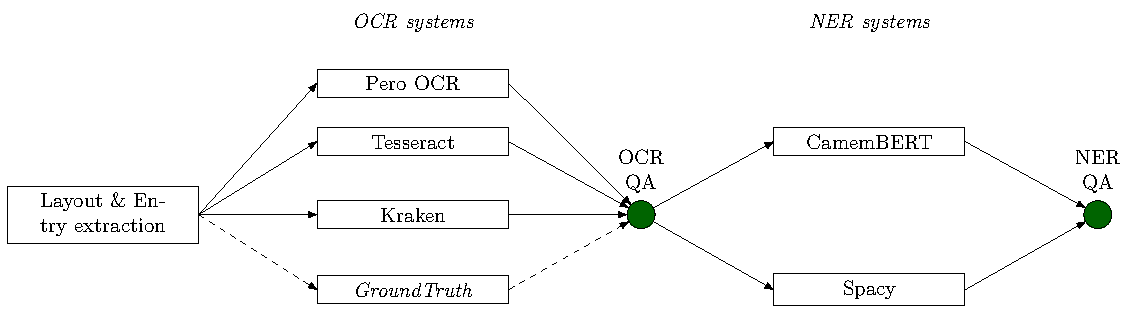
\includegraphics[width=\linewidth]{figs/protocol.pdf}
    \caption{Scheme of the evaluation protocol. \joseph{Missing "Ground truth" for NER stage?}}
    \label{fig.protocol}
    \end{figure}


